\documentclass[14pt,aspectratio=1610]{beamer}
\usepackage[T1]{fontenc}
\usepackage[utf8]{inputenc}
\usepackage[ngerman]{babel}
\uselanguage{ngerman}
\languagepath{ngerman}
\usetheme{simple}
\usecolortheme{whiteonblack}
\usepackage{listings}
%\usepackage{aurl}
%\daurl{meta}{http://www.snik.eu/ontology/meta/}
%\daurl{ob}{http://www.snik.eu/ontology/ob/}
%\daurl{bb}{http://www.snik.eu/ontology/bb/}
\usepackage{url}
\usepackage{graphicx}
%\date{25. März 2022}
\title{SHACL}
\subtitle{Shapes Constraint Language}
\begin{document}

\begin{frame}
\titlepage
\end{frame}

\begin{frame}{}
\centering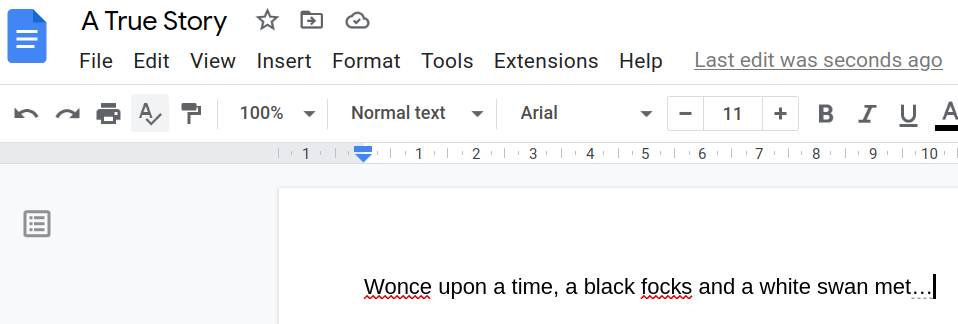
\includegraphics[width=1.05\textwidth,height=1.05\textheight,keepaspectratio]{img/spelling.png}
\end{frame}

\begin{frame}{}
\centering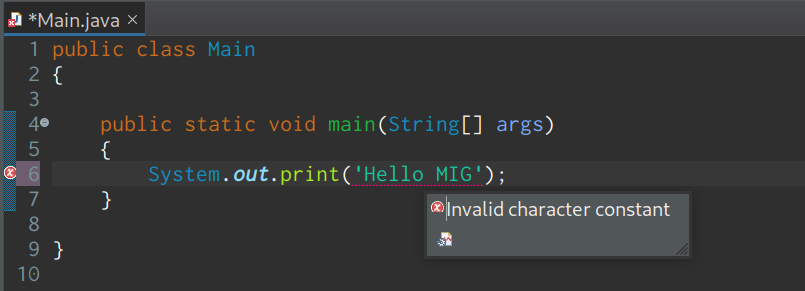
\includegraphics[width=1.05\textwidth,height=1.05\textheight,keepaspectratio]{img/javaerror.png}
\end{frame}

\begin{frame}{}
\centering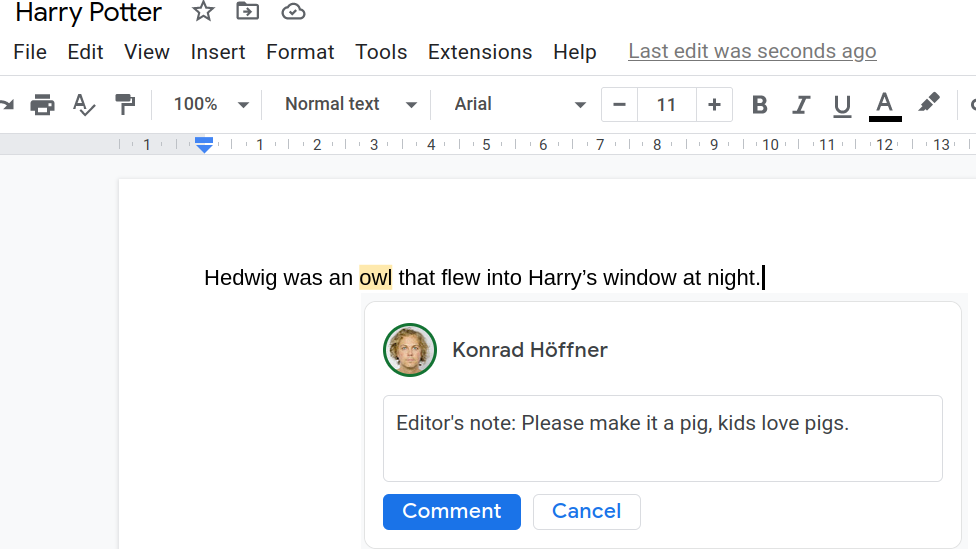
\includegraphics[width=1.05\textwidth,height=1.05\textheight,keepaspectratio]{img/hedwig.png}
\end{frame}

% some images unfortunately not commited and lost, comment them out
%\begin{frame}{}
%\centering\includegraphics[width=1.05\textwidth,height=1.05\textheight,keepaspectratio]{img/java-hedwig-owl.png}
%\end{frame}

%\begin{frame}{}
%\centering\includegraphics[width=1.05\textwidth,height=1.05\textheight,keepaspectratio]{img/java-hedwig-pig.png}
%\end{frame}

\begin{frame}{}
\centering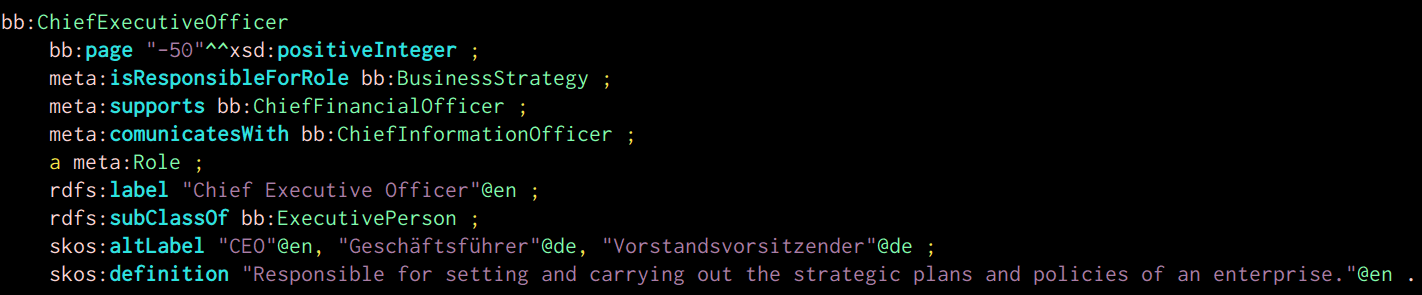
\includegraphics[width=1.05\textwidth,height=1.05\textheight,keepaspectratio]{img/bb-ceo.png}
\end{frame}

%\begin{frame}{}
%\centering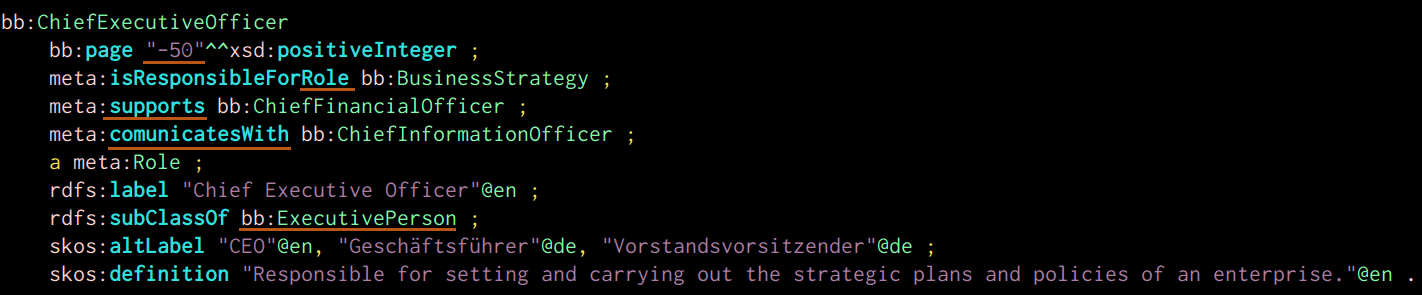
\includegraphics[width=1.05\textwidth,height=1.05\textheight,keepaspectratio]{img/bb-ceo-marked.png}
%\end{frame}

%\begin{frame}{}
%\centering\includegraphics[width=1.05\textwidth,height=1.0\textheight,keepaspectratio]{img/SNIK\_Metamodell\_V8.pdf}
%\end{frame}

%\begin{frame}[fragile]{}
%:Role
%    a owl:Class ;
%    rdfs:label "Rolle"@de, "role"@en ;  
%    rdfs:subClassOf :Top ;
%    owl:disjointWith :EntityType, :Function .
%
%:communicatesWith
%    a owl:ObjectProperty ; 
%    rdfs:domain :ApplicationComponent ;
%    rdfs:label "communicates with"@en ;
%    rdfs:range :ApplicationComponent .
%}
%\end{frame}

\begin{frame}[fragile]{Hedwig the Owl}
\small
\begin{lstlisting}
@prefix rdfs: <http://www.w3.org/2000/01/rdf-schema#> .
@prefix owl: <http://www.w3.org/2002/07/owl#>.
@prefix : <http://example.com/> .

# Ontology (T-Box)
:Owl a owl:Class.
:Pig a owl:Class.
:fliesTo a owl:ObjectProperty; rdfs:domain :Owl.

# Knowledge Base (A-Box)
:hedwig a :Owl; :fliesTo :London.
\end{lstlisting}
\end{frame}

\begin{frame}[fragile]{Hedwig the Owl---Reasoner}
\small
\begin{lstlisting}
:Owl a rdfs:Class, rdfs:Resource, owl:Class,owl:Thing ;
    rdfs:subClassOf :Owl, rdfs:Resource, owl:Thing ;
    owl:equivalentClass :Owl ;
    owl:sameAs :Owl .

:Pig a rdfs:Class,
        rdfs:Resource, owl:Class, owl:Thing ;
    rdfs:subClassOf :Pig, rdfs:Resource, owl:Thing ;
    owl:equivalentClass :Pig ;
    owl:sameAs :Pig .
[...]
\end{lstlisting}
\end{frame}

\begin{frame}[fragile]{Hedwig the Pig}
\small
\begin{lstlisting}
@prefix rdfs: <http://www.w3.org/2000/01/rdf-schema#> .
@prefix owl: <http://www.w3.org/2002/07/owl#>.
@prefix : <http://example.com/> .

# Ontology (T-Box)
:Owl a owl:Class.
:Pig a owl:Class.
:fliesTo a owl:ObjectProperty; rdfs:domain :Owl.

# Knowledge Base (A-Box)
:hedwig a :Pig; :fliesTo :London.
\end{lstlisting}
\end{frame}

\begin{frame}[fragile]{Hedwig the Pig---Reasoner}
\begin{lstlisting}
:hedwig a :Owl,
        :Pig,
        rdfs:Resource,
        owl:Thing ;
    :fliesTo :London ;
    owl:sameAs :hedwig .
\end{lstlisting}
\end{frame}

\begin{frame}[fragile]{owl:disjointWith hilft nicht}
\small
\begin{lstlisting}
@prefix rdfs: <http://www.w3.org/2000/01/rdf-schema#> .
@prefix owl: <http://www.w3.org/2002/07/owl#>.
@prefix : <http://example.com/> .

# Ontology (T-Box)
:Owl a owl:Class.
:Pig a owl:Class; owl:disjointWith :Owl.
:fliesTo a owl:ObjectProperty; rdfs:domain :Owl.

# Knowledge Base (A-Box)
:hedwig a :Pig; :fliesTo :London.
\end{lstlisting}
\end{frame}

\begin{frame}[fragile]{SHACL}
\small
\begin{lstlisting}
@prefix : <http://example.com/>.
@prefix owl: <http://www.w3.org/2002/07/owl#>.
@prefix rdf: <http://www.w3.org/1999/02/22-rdf-syntax-ns#>.
@prefix sh: <http://www.w3.org/ns/shacl#>.

:OwlShape a sh:NodeShape;
    sh:targetClass :Owl;    
    sh:property [sh:path :fliesTo].

:PigShape a sh:NodeShape;
    sh:targetClass :Pig.

:fliesToRangeShape a sh:NodeShape;                  
    sh:targetObjectsOf :fliesTo;        
    sh:class :Owl.
\end{lstlisting}
\end{frame}

\begin{frame}[fragile]{pySHACL}
\small
\begin{lstlisting}
pyshacl -s shacl.ttl hedwig.ttl

Validation Report
Conforms: False
Results (1):
Constraint Violation in ClassConstraintComponent (http://www.w3.org/ns/shacl#ClassConstraintComponent):
	Severity: sh:Violation
	Source Shape: :fliesToRangeShape
	Focus Node: :London
	Value Node: :London
	Message: Value does not have class :Owl
\end{lstlisting}
\end{frame}

\begin{frame}{Links}
\begin{itemize}
\item \url{https://www.w3.org/TR/shacl/}
\item \url{https://www.ldf.fi/service/owl-rl-reasoner}
\item \url{https://github.com/konradhoeffner/shacl}
\end{itemize}
\end{frame}

\end{document}
